\documentclass[tikz, border=12pt]{standalone}
\usepackage{amsmath}
\usepackage{tikz}
\usetikzlibrary{shapes.geometric, arrows.meta, positioning, fit, backgrounds}

% ── Styles ────────────────────────────────────────────────────────────────────
\tikzset{
  startstop/.style={
    rectangle, rounded corners=8pt,
    minimum width=4.2cm, minimum height=1cm,
    text centered, draw=black, thick,
    fill=black!75, text=white, font=\bfseries
  },
  process/.style={
    rectangle, rounded corners=4pt,
    minimum width=5.2cm, minimum height=1cm,
    text centered, draw=black!70, thick,
    fill=blue!12, font=\small
  },
  decision/.style={
    diamond, aspect=2.8,
    minimum width=5.4cm, minimum height=1cm,
    text centered, draw=black!70, thick,
    fill=orange!20, font=\small
  },
  output/.style={
    rectangle, rounded corners=4pt,
    minimum width=5.2cm, minimum height=1cm,
    text centered, draw=black!60, thick,
    fill=green!14, font=\small
  },
  rule/.style={
    rectangle, rounded corners=3pt,
    minimum width=7.5cm, minimum height=0.85cm,
    text centered, draw=red!55, thick,
    fill=red!8, font=\small
  },
  aggregate/.style={
    rectangle, rounded corners=4pt,
    minimum width=5.2cm, minimum height=1cm,
    text centered, draw=gray!60, thick,
    fill=gray!10, font=\small
  },
  arrow/.style={-{Stealth[length=7pt]}, thick, draw=black!60},
}

\begin{document}
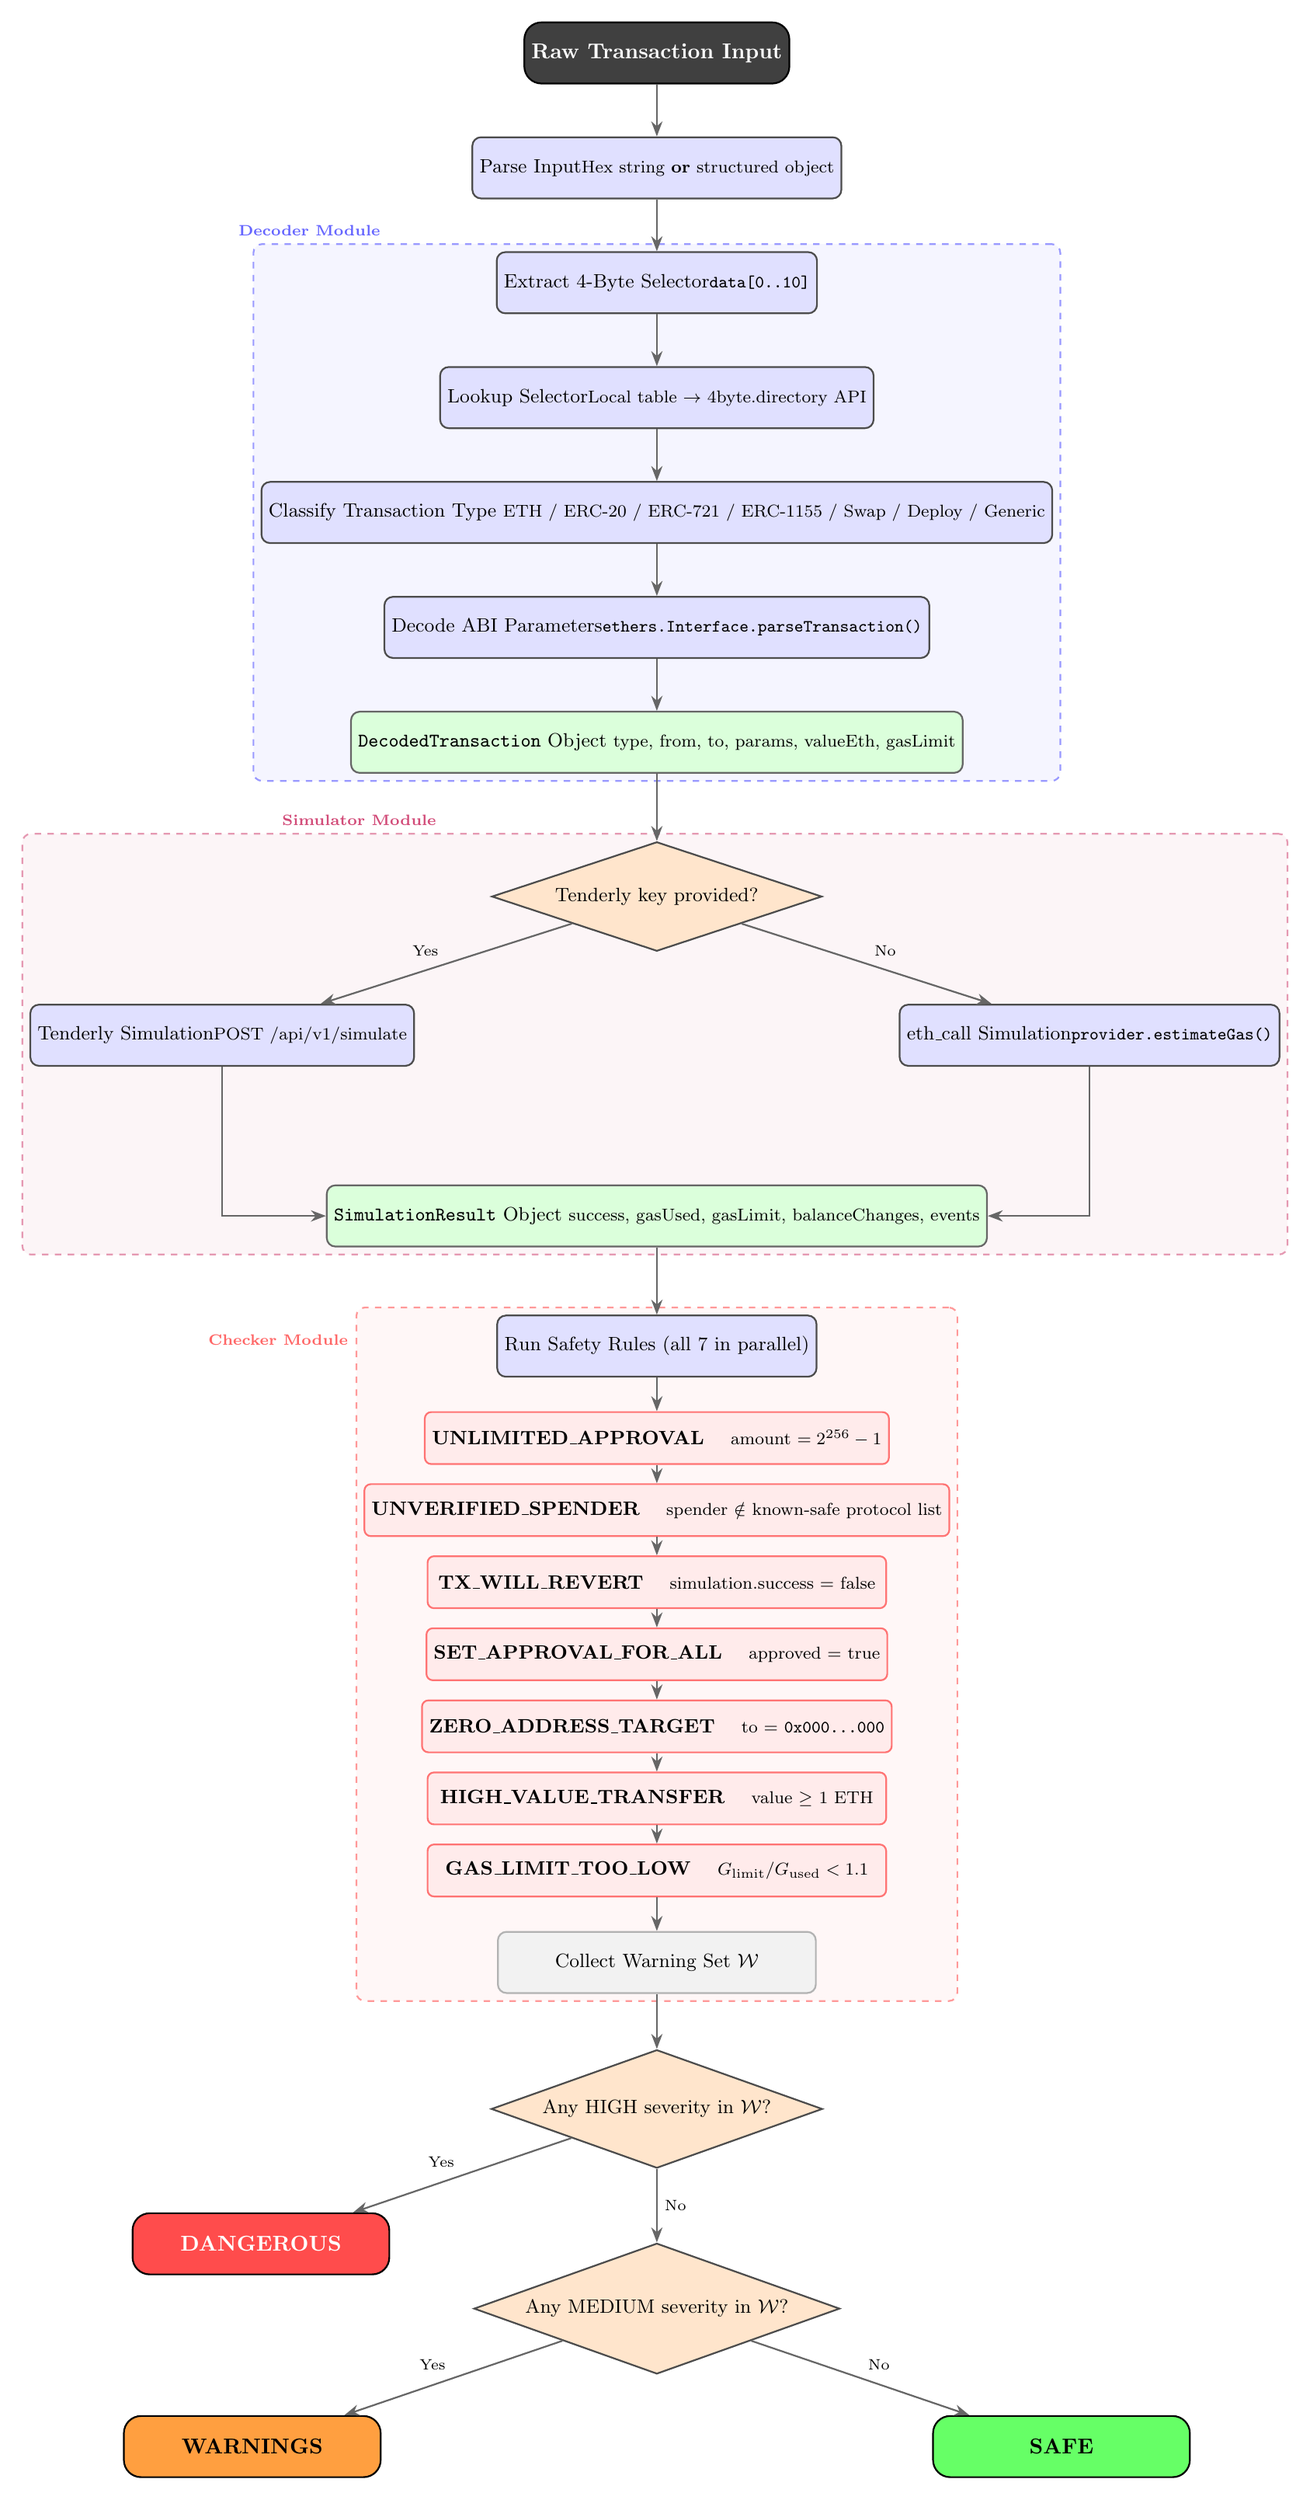
\begin{tikzpicture}[node distance=0.85cm]

% ── INPUT ─────────────────────────────────────────────────────────────────────
\node (start) [startstop]
  {Raw Transaction Input};

\node (inputtype) [process, below=of start]
  {Parse Input\\[-2pt]{\footnotesize Hex string \textbf{or} structured object}};

% ── DECODER ──────────────────────────────────────────────────────────────────
\node (selector) [process, below=of inputtype]
  {Extract 4-Byte Selector\\[-2pt]{\footnotesize \texttt{data[0..10]}}};

\node (lookup) [process, below=of selector]
  {Lookup Selector\\[-2pt]{\footnotesize Local table $\rightarrow$ 4byte.directory API}};

\node (classify) [process, below=of lookup]
  {Classify Transaction Type\\[-2pt]
   {\footnotesize ETH / ERC-20 / ERC-721 / ERC-1155 / Swap / Deploy / Generic}};

\node (params) [process, below=of classify]
  {Decode ABI Parameters\\[-2pt]{\footnotesize \texttt{ethers.Interface.parseTransaction()}}};

\node (decoded) [output, below=of params]
  {\texttt{DecodedTransaction} Object\\[-2pt]
   {\footnotesize type, from, to, params, valueEth, gasLimit}};

% ── SIMULATOR ────────────────────────────────────────────────────────────────
\node (simroute) [decision, below=1.1cm of decoded]
  {Tenderly key provided?};

\node (tenderly) [process, below left=1.3cm and 2.6cm of simroute]
  {Tenderly Simulation\\[-2pt]{\footnotesize POST /api/v1/simulate}};

\node (rpc) [process, below right=1.3cm and 2.6cm of simroute]
  {eth\_call Simulation\\[-2pt]{\footnotesize \texttt{provider.estimateGas()}}};

\node (simresult) [output, below=3.8cm of simroute]
  {\texttt{SimulationResult} Object\\[-2pt]
   {\footnotesize success, gasUsed, gasLimit, balanceChanges, events}};

% ── CHECKER : single-column rule list ────────────────────────────────────────
\node (checks) [process, below=1.1cm of simresult]
  {Run Safety Rules (all 7 in parallel)};

\node (r1) [rule, below=0.55cm of checks]
  {\textbf{UNLIMITED\_APPROVAL} \quad {\footnotesize amount $= 2^{256}-1$}};

\node (r2) [rule, below=0.3cm of r1]
  {\textbf{UNVERIFIED\_SPENDER} \quad {\footnotesize spender $\notin$ known-safe protocol list}};

\node (r3) [rule, below=0.3cm of r2]
  {\textbf{TX\_WILL\_REVERT} \quad {\footnotesize simulation.success $=$ false}};

\node (r4) [rule, below=0.3cm of r3]
  {\textbf{SET\_APPROVAL\_FOR\_ALL} \quad {\footnotesize approved $=$ true}};

\node (r5) [rule, below=0.3cm of r4]
  {\textbf{ZERO\_ADDRESS\_TARGET} \quad {\footnotesize to $=$ \texttt{0x000\ldots000}}};

\node (r6) [rule, below=0.3cm of r5]
  {\textbf{HIGH\_VALUE\_TRANSFER} \quad {\footnotesize value $\geq$ 1 ETH}};

\node (r7) [rule, below=0.3cm of r6]
  {\textbf{GAS\_LIMIT\_TOO\_LOW} \quad
   {\footnotesize $G_{\mathrm{limit}} / G_{\mathrm{used}} < 1.1$}};

% ── AGGREGATE ────────────────────────────────────────────────────────────────
\node (agg) [aggregate, below=0.55cm of r7]
  {Collect Warning Set $\mathcal{W}$};

% ── SCORE ────────────────────────────────────────────────────────────────────
\node (score) [decision, below=0.9cm of agg]
  {Any HIGH severity in $\mathcal{W}$?};

\node (danger) [startstop, below left=1.2cm and 3.0cm of score, fill=red!70]
  {DANGEROUS};

\node (anywarn) [decision, below=1.2cm of score]
  {Any MEDIUM severity in $\mathcal{W}$?};

\node (warnings) [startstop, below left=1.2cm and 3.0cm of anywarn,
                  fill=orange!75, text=black]
  {WARNINGS};

\node (safe) [startstop, below right=1.2cm and 3.0cm of anywarn,
              fill=green!60, text=black]
  {SAFE};

% ── ARROWS: Input → Decode ───────────────────────────────────────────────────
\draw [arrow] (start)     -- (inputtype);
\draw [arrow] (inputtype) -- (selector);
\draw [arrow] (selector)  -- (lookup);
\draw [arrow] (lookup)    -- (classify);
\draw [arrow] (classify)  -- (params);
\draw [arrow] (params)    -- (decoded);

% ── ARROWS: Decode → Simulate ────────────────────────────────────────────────
\draw [arrow] (decoded)  -- (simroute);
\draw [arrow] (simroute) -- node[above left,  font=\scriptsize]{Yes} (tenderly);
\draw [arrow] (simroute) -- node[above right, font=\scriptsize]{No}  (rpc);
\draw [arrow] (tenderly) |- (simresult);
\draw [arrow] (rpc)      |- (simresult);

% ── ARROWS: Simulate → Checker ───────────────────────────────────────────────
\draw [arrow] (simresult) -- (checks);
\draw [arrow] (checks) -- (r1);
\draw [arrow] (r1) -- (r2);
\draw [arrow] (r2) -- (r3);
\draw [arrow] (r3) -- (r4);
\draw [arrow] (r4) -- (r5);
\draw [arrow] (r5) -- (r6);
\draw [arrow] (r6) -- (r7);
\draw [arrow] (r7) -- (agg);

% ── ARROWS: Aggregate → Score ────────────────────────────────────────────────
\draw [arrow] (agg)     -- (score);
\draw [arrow] (score)   -- node[above left,  font=\scriptsize]{Yes} (danger);
\draw [arrow] (score)   -- node[right,        font=\scriptsize]{No}  (anywarn);
\draw [arrow] (anywarn) -- node[above left,  font=\scriptsize]{Yes} (warnings);
\draw [arrow] (anywarn) -- node[above right, font=\scriptsize]{No}  (safe);

% ── MODULE GROUPING ──────────────────────────────────────────────────────────
\begin{pgfonlayer}{background}
  \node[draw=blue!40, fill=blue!4, rounded corners, thick, dashed,
        fit=(selector)(lookup)(classify)(params)(decoded),
        label={[font=\scriptsize\bfseries, blue!60]above left:Decoder Module}] {};

  \node[draw=purple!40, fill=purple!4, rounded corners, thick, dashed,
        fit=(simroute)(tenderly)(rpc)(simresult),
        label={[font=\scriptsize\bfseries, purple!70]above left:Simulator Module}] {};

  \node[draw=red!40, fill=red!3, rounded corners, thick, dashed,
        fit=(checks)(r1)(r2)(r3)(r4)(r5)(r6)(r7)(agg),
        label={[font=\scriptsize\bfseries, red!60]above left:Checker Module}] {};
\end{pgfonlayer}

\end{tikzpicture}
\end{document}
